%%%%%%%%%%%%%%%%%%%%%%%%%%%%%%%%%%%%%%%%%%%%%%%%%%%%%%%%%%%%%%%%%%%%%%%%%%%%%%%%%%%%%%%%%%%%%%%%%%%%%%%%%%%%%%%%%%%%%%%%%%%%%%%%%%%%%%%%
% This is just a template to use when submitting manuscripts to Frontiers, it is not mandatory to use frontiers.cls nor frontiers.tex  %
%%%%%%%%%%%%%%%%%%%%%%%%%%%%%%%%%%%%%%%%%%%%%%%%%%%%%%%%%%%%%%%%%%%%%%%%%%%%%%%%%%%%%%%%%%%%%%%%%%%%%%%%%%%%%%%%%%%%%%%%%%%%%%%%%%%%%%%%

\documentclass{frontiersSCNS} % for Science articles
%\documentclass{frontiersMED} % for Medicine articles

\usepackage{url}

%\usepackage{lineno}
\usepackage{todonotes}


% Absolute numerotation for figures
\usepackage{caption}
%\usepackage{subcaption}
\captionsetup{figurewithin=none}  
\captionsetup{tablewithin=none}
%\usepackage[tight]{subfigure}
\def\subfigbottomskip{0pt}

\usepackage{listings}
\lstset{language=python,
	basicstyle=\ttfamily,
	extendedchars=true,
	xleftmargin = 0pt,
	rulecolor=\color{black!50},
        aboveskip = 0.5ex,
        belowskip = 0.6ex,
	escapebegin={\color{green!50!black}},
        %keywordstyle=\sffamily\bfseries\color{grey},
	%identifierstyle=\sffamily,
	commentstyle=\slshape\color{green!50!black},
	stringstyle=\rmfamily\color{blue},
	showstringspaces=false,
	tabsize=2,
	breaklines=true,
	%classoffset=1,
        morekeywords={{,},=,:},
	%classoffset=0,
        frame=single,xleftmargin=\fboxsep,xrightmargin=-\fboxsep
    }
	

%\makeatletter
% Space between floats
%\setlength\floatsep    {4\p@}
% Space between floats and text
%\setlength\textfloatsep{4\p@}
% Space above and below an inline figure
%\setlength\intextsep   {4\p@}
%\makeatother


\newcommand{\alex}[1]{\todo[inline, color=green!40]{#1}}
\newcommand{\fabian}[1]{\todo[inline, color=blue!40]{#1}}
\newcommand{\bertrand}[1]{\todo[inline, color=red!40]{#1}}
\newcommand{\michael}[1]{\todo[inline, color=yellow!40]{#1}}


%\linenumbers


\copyrightyear{}
\pubyear{}
%\onecolumn
%%% write here for which journal %%%
\def\journal{Neurosciences}
\def\DOI{}
\def\articleType{}
\def\citing{\color{darkgray}\cite}
\def\keyFont{\fontsize{6}{11}\helveticabold }
\def\firstAuthorLast{Alexandre Abraham {et~al}} %use et al only if is more than 1 author

% XXX Review the order of authors

\def\Authors{
    Alexandre Abraham\,$^{1,2,*}$,
    Fabian Pedregosa\,$^{1,2}$,
    Michael Eickenberg\,$^{1,2}$,
    Philippe Gervais\,$^{1,2}$,
    Andreas Muller\,$^{3}$,
    Jean Kossaifi\,$^{4}$,
    Alexandre Gramfort\,$^{1,2,5}$,
    Bertrand Thirion\,$^{1,2}$
    and Ga\"el Varoquaux\,$^{1,2}$}
% Affiliations should be keyed to the author's name with superscript numbers and be listed as follows: Laboratory, Institute, Department, Organization, City, State abbreviation (USA, Canada, Australia), and Country (without detailed address information such as city zip codes or street names).
% If one of the authors has a change of address, list the new address below the correspondence details using a superscript symbol and use the same symbol to indicate the author in the author list.
\def\Address{
    $^{1}$Parietal Team, INRIA Saclay-\^{I}le-de-France, Saclay, France\\
    $^{2}$Neurospin, I\,\textsuperscript{2}BM, DSV, CEA, 91191 Gif-Sur-Yvette, France\\
    $^{3}$Institute of Computer Science VI, University of Bonn, Germany\\
    $^{4}$Department of Computing, Imperial College London, U.K.\\
    $^{5}$Institut Mines-Telecom, Telecom ParisTech, CNRS LTCI, 75014 Paris, France}

% The Corresponding Author should be marked with an asterisk
% Provide the exact contact address (this time including street name and city zip code) and email of the corresponding author
\def\corrAuthor{Alexandre Abraham}
\def\corrAddress{Parietal Team, INRIA Saclay-\^{I}le-de-France, Saclay, France}
\def\corrEmail{alexandre.abraham@inria.fr}

% \color{FrontiersBlue} Is the blue color, used in the Journal name, in the title, and the names of the sections

% Bunch of code for 3D cubes

% Example of table from template

% \begin{table}[!t]
% \processtable{Resolution Requirements for the figures\label{Tab:01}}
% {\begin{tabular}{lllll}\toprule
% Image Type & Description & Format & Color Mode & Resolution\\\midrule
% Line Art & An image composed of lines and text,  & TIFF, EPS, JPEG & RGB, Bitmap & 900 - 1200 dpi\\
%            & which does not contain tonal or shaded areas.& & &\\
%            Halftone & A continuous tone photograph, which contains no text. & TIFF, EPS, JPEG & RGB, Grayscale & 300 dpi\\
% Combination & Image contains halftone + text or line art elements. & TIFF, EPS, JPEG & RGB,Grayscale & 600 - 900 dpi\\\botrule
% \end{tabular}}{This is a footnote}
% \end{table}


% Figures

% \textbf{Figure 1.}{ Enter the caption for your figure here.  Repeat as  necessary for each of your figures.}\label{fig:01}
% Don't add the figures in the LaTeX files, please upload them when submitting the article. Frontiers will add the figures at the end of the provisional pdf.


%%%%%%%%%%%%%%%%%%%%%%%%%%%%%%%%%%%%%%%%%%%%%%%%%%%%%%%%%%%%%%%%%%%%%%%%%%%%%%%
%%%%%%%%%%%%%%%%%%%%%%%%%%%%%%%%%%%%%%%%%%%%%%%%%%%%%%%%%%%%%%%%%%%%%%%%%%%%%%%
%%%%                                                                       %%%%
%%%%                          Naming convention                            %%%%
%%%%                                                                       %%%%
%%%%%%%%%%%%%%%%%%%%%%%%%%%%%%%%%%%%%%%%%%%%%%%%%%%%%%%%%%%%%%%%%%%%%%%%%%%%%%%
%%%%%%%%%%%%%%%%%%%%%%%%%%%%%%%%%%%%%%%%%%%%%%%%%%%%%%%%%%%%%%%%%%%%%%%%%%%%%%%

% Nifti world
% -----------
% - func_filename: name of a dataset file
% - func_img: name of a (loaded) nifti file
% - func_data, func_affine: data and affine of functional data

% Scikit-learn world
% ------------------
% - Xs: list of unmasked func_data (scikit-learn world)
% - X: unmasked func_data reduced to 2 dimensions (scikit-learn world)
% - y: labels

\begin{document}
\onecolumn
\firstpage{1}

\title[Machine Learning for Neuroimaging with Scikit-Learn]{Machine Learning for Neuroimaging with Scikit-Learn}
\author[\firstAuthorLast ]{\Authors}
\address{}
\correspondance{}
\editor{}
\topic{Research Topic}

\maketitle
\begin{abstract}

\section{}
Statistical machine learning methods are increasingly used for
neuroimaging data analysis. Their main virtue for this type of application
is their ability to model high-dimensional datasets, e.g.\ multivariate
analysis of activation images, or capturing inter-subject variability.
Supervised learning is typically used in \emph{decoding} or
\emph{encoding} settings to relate
brain images to behavioral or clinical observations, while
unsupervised learning is typically used to uncover hidden structure in
sets of images (e.g.\ resting state functional MRI) or to find
sub-populations in large cohorts of subjects. By considering
different functional neuroimaging applications, we illustrate how scikit-learn,
a Python machine learning library, can be used to perform some key
analysis steps. Scikit-learn contains a large set of statistical
learning algorithms, both supervised and unsupervised, that can be applied
to neuroimaging data. Other Python libraries provide the tools for
loading and preparing neuroimaging data for scikit-learn, and visualizing
the results.

% XXX: here the tone of the article should be: scikit-learn for methods
% development, ie we target the methods researchers for Neuroimaging. We
% should make this explicit in the intro and conclusion

\tiny
% XXX Fix keywords
%All article types: you may provide up to 8 keywords; at least 5 are mandatory.
\section{Keywords:} machine learning, statistical learning, neuroimaging,
scikit-learn, Python
\end{abstract}


\section{Introduction}

Statistical machine learning is gaining interest in
neuroimaging data analysis. It is used by neuroscientists as a complicated
yet powerful tool for statistical inference,
and by computer scientists working in neuroscience,
who often lack a deep understanding of the neuroscience questions. This paper
aims to fill the gap between machine learning and neuroimaging by demonstrating
how a general-purpose machine-learning toolbox can be used to produce scripts 
for neuroimaging analysis with state-of-the-art methods
that are fully understood by both worlds. For a more theoretical introduction to
the use of machine learning methods for functional MRI analysis, see
\cite{pereira2009} or \cite{mur2009}.

With its mature scientific stack, Python is a growing contender in the
landscape of neuroimaging data analysis with tools such as Nipy
\citep{millman2007analysis} or Nipype \citep{gorgolewski2011}.
For multi-variate pattern analysis, PyMVPA \citep{hanke2009pymvpa}
combines Python and external tools such as R or Shogun
\citep{sonnenburg2010}. 

In this paper, we show how scikit-learn, a Python machine learning
library \citep{pedregosa2011}, can be used on neuroimaging data.
We discuss a few applications of statistical learning to
resolve common neuroimaging needs, which methods can be used, what the underlying
assumptions are, and how to achieve the desired results. We discuss not only
prediction scores, but also the interpretability of the results, which
leads us to explore the internal model of various methods. 
The scope of this paper is not to discuss a library, but rather
code patterns, and the github repository of the
paper\footnote{\url{http://www.github.com/AlexandreAbraham/frontiers2013}}
provides complete scripts to generate figures. Naturally, there would be
value in a software package building upon these patterns. Such a package
is under development, in the form of nilearn
--\url{http://nilearn.github.io}-- but is, to date, not ready
for public consumption.

The paper is organized as
follows. After introducing the \emph{scikit-learn} toolbox, we show 
how the data must be prepared to apply
\emph{scikit-learn}. Then we describe the application of \emph{supervised
learning} techniques, to learn the links between brain images and
stimuli. Finally we demonstrate how \emph{unsupervised learning}
techniques can extract useful structure from the images.

% Maybe we should stress that this paper is meant to be didactic, and
% thus only presents simple examples

\subsection{Scientific Python and neuroimaging ecosystem}

Thanks to its scientific libraries, Python is able to compete with domain-specific
languages such as Matlab or R. The main libraries in the scientific Python stack are:
\begin{itemize}
    \item{\bf NumPy} provides the \verb!ndarray! data type, an efficient $n$-dimensional data
        representation for array-based numerical computating, a la Matlab
        \citep{vanderwalt2011}. It handles efficient NumPy array persistance
        (input and output) and provides basic operations such as dot product. A
        growing number of scientific libraries, including scikit-learn, uses NumPy arrays
        as input and output data type. Section~\ref{data_preparation} explains
        how to load neuroimaging data and convert it to NumPy arrays compatible
        with scikit-learn.

    \item{\bf SciPy} provides higher level mathematical functions that operate on ndarrays for
        a variety of domains including linear algebra, optimization and signal
        processing. SciPy is linked to compiled libraries to ensure high
        performances (BLAS, Arpack and MKL for linear algebra and mathematical
        operations and libSVM and libLinear for SVM).
        Together, NumPy and SciPy provide a robust scientific environment
        for numerical computing and they are the elementary bricks we use in all our
        algorithms.
        % XXX : elementary bricks -> foundations ? building blocks?

    \item{\bf Matplotlib} is a plotting library tightly integrated into the
        scientific Python stack \citep{hunter2007}. It offers publication-quality figures in
        a variety of formats.
        %  and can display plots or images in a
        % graphical user interface.
        All figures in this paper have been generated with it.

    \item{\bf Nibabel} loads or saves data in neuroimaging file formats.
	We use it at the beginning of all our scripts.
\end{itemize}

\subsection{Scikit-learn and machine learning ecosystem}

Scikit-learning is a general purpose machine learning library written in Python.
It proposes efficient implementations of state-of-the-art algorithms. It also
takes advantage of Python interactivity and modularity to propose fast and easy
prototyping.

Weka \citep{hall2009weka}, a machine learning framework written in Java,
provides a simple user interface, however it is more oriented toward data mining
and it using its API for specific purpose requires knowledge of the
Java Runtime Environment. PyBrain \citep{schaul2010pybrain} is best at neural networks
and reinforcement learning approaches, which are black boxes, and does not match
our will to interpret the results.

Some higher level frameworks provides full pipeline to apply machine learning techniques on
neuroimaging data. PyMVPA does data preprocessing, analysis and result
visualization, but has dependencies on R and Shogun. PRoNTo
\citep{schrouff2013pronto} is written in Matlab and can easily interface with
SPM but does not propose many machine learning algorithms. This paper is about
patterns that are lower-level.

\section{Scikit-learn}
\label{scikitlearn}

{\em Scikit-learn} \citep{pedregosa2011} is an open source machine
learning library for the Python programming language. The ambition of the
project is to provide efficient and well-established machine learning tools within
a programming environment accessible to non-machine learning experts
and reusable across scientific disciplines and applicative fields.

\subsection{Concepts}

In {\em scikit-learn}, all objects and algorithms accept input data in the form of
2-dimensional arrays of size samples $\times$ features.
This convention makes it generic and domain-independent.
Scikit-learn objects share a uniform set of methods that
depends on their purpose: \textit{estimators} can fit models from data,
\textit{predictors} can make predictions on new data and \textit{transformers}
convert data from one representation to another.

\begin{itemize}
\item {\bf Estimator}. The \textit{estimator} interface, the core of the
    library, exposes a \texttt{fit} method for learning model parameters from training data.
    All supervised
    and unsupervised learning algorithms (e.g., for classification, regression or
    clustering) are available as objects implementing this interface. Machine
    learning tasks such as feature extraction, feature selection or dimensionality
    reduction are also provided as estimators.

\item {\bf Predictor}. The \textit{predictor} interface extends the notion of an estimator
    by adding a \texttt{predict}
    method that takes an input array \texttt{X\_test} and makes
    predictions for each sample in it.
    We call the input parameter ``\texttt{X\_test}'' in order
    to emphasize that \texttt{predict} generalizes to new data. In the case of
    supervised learning estimators, this method typically returns the predicted
    labels or values computed from the estimated model.

\item {\bf Transformer}. As it is common to modify or filter data before feeding it to a learning
    algorithm, some estimators, named \textit{transformers}, implement a
    \texttt{transform} method. Preprocessing, feature selection and
    dimensionality reduction
    algorithms are all provided as transformers within the library. If the transformation
    can be inverted, a method called \texttt{inverse\_transform} also exists.

\end{itemize}

\subsection{Cross-validation and model selection}

% XXX: describe cross-validation
When testing an estimator or setting hyperparameters, one needs a reliable
metric to evaluate its performance. Using the same
data for training and testing is not acceptable because it leads to
overly confident model performance, a phenomenon also known as \emph{overfitting}.
Cross-validation is a technique that allows one to reliably evaluate an
estimator on a given dataset. It consists in iteratively fitting the
estimator on a fraction of the data, called \emph{training set}, and testing it
on the left-out unseen data, called \emph{test set}.
Several strategies exists to partition the data.
For example, K-Fold cross validation consists in dividing (randomly or not) the samples in $k$
subsets: each subset is then used once as testing set while the others $k - 1$
subsets are used to train the estimator. This is one of the simplest and most
widely used cross-validation strategies. The parameter $k$ is commonly set
to 5 or 10. Other strategies, sometimes called Monte-Carlo cross-validation,
use many random partitions in the data.

For a given model and some fixed value of hyperparameters, the scores
on the various test sets can be averaged to give a quantitative score
to assess how good the model is. Maximizing this cross-validation score offers
a principled way to set hyperparameters and allows to choose between
different models. This procedure is known as \emph{model selection}.
%
In {\em scikit-learn}, hyperparameters tuning can be conviently done with the
\texttt{GridSearchCV} estimator. It takes as input an estimator and
a set of candidate hyperparameters. Cross-validation scores are then
computed for all hyperparameters combinations, possibly in parallel,
in order to find the best one. In this paper, we set the regularization
coefficient with grid search in section~\ref{kamitani}.

\section{Data preparation: from MR volumes to a data matrix}
\label{data_preparation}
Before applying statistical learning to neuroimaging data, standard
preprocessing must be applied. For fMRI, this includes motion
correction, slice timing correction, coregistration with an anatomical image and normalization to a common
template like the MNI (Montreal Neurologic Institute) one if necessary.
Reference softwares for these tasks are
SPM\footnote{http://www.fil.ion.ucl.ac.uk/spm}~\citep{friston2007} and
FSL\footnote{http://fsl.fmrib.ox.ac.uk}~\citep{smith2004}. A Python
interface to these tools is available in nipype Python library
\citep{gorgolewski2011}. Below we discuss shaping preprocessed data into
a format that can be fed to scikit-learn. For the machine learning
settings, we need a data matrix, that we will denote $X$, and optionally a
target variable to predict, $y$.

\subsection{Spatial resampling}
\label{resampling}

Neuroimaging data often come as Nifti files, 4-dimensional data (3D scans
with time series at each location or voxel) along with a
transformation matrix (called affine) used to compute voxel locations
from array indices to world coordinates. When working with several subjects,
each individual data is registered on a common template (MNI, Talairach...),
hence on a common affine, during preprocessing.

Affine matrix can express data
anisotropy, when the distance between two voxels is not the same
depending on the direction. This information is used by algorithms
relying on the spatial structure of the data, for instance the
Searchlight.

SciPy routine \texttt{scipy.ndimage.affine\_transform}
can be used to perform image resampling: 
changing the spatial resolution of the data\footnote{An easy-to-use
implementation is proposed in nilearn}. This is
an interpolation and alters the data, that is why it should be used carefully.
Downsampling is commonly used to reduce the size of data to process.
Typical sizes are 2mm or 3mm resolution, but scan spatial resolution is
increasing with progress in MR physics. The affine matrix can encode the
scaling factors for each direction.

\subsection{Signal cleaning}

Due to its complex and indirect acquisition process, neuroimaging data often has a low
signal-to-noise ratio. It contains trends and artifacts that must be removed
to ensure maximum machine learning algorithms efficiency. Signal cleaning
includes:
\begin{itemize}
    \item{\bf Detrending} removes a linear trend over the time series of each
        voxel. This is a useful step when studying fMRI data, as the voxel
        intensity itself has no meaning and we want to study its variation and
        correlation with other voxels. Detrending can be done thanks to SciPy
        (\texttt{scipy.signal.detrend}).
% bzw, linear detrending is utterly insufficient
% That's why we do low pass
    \item{\bf Normalization} consists in setting the timeseries variance to 1.
        This harmonization is necessary as some machine learning algorithms are
        sensible to different value ranges.
    \item{\bf Frequency filtering} consists in removing high or low
        frequency signals. Low-frequency signals in fMRI data are caused by
        physiological mechanisms or scanner drifts. Filtering can be done thanks
        to a Fourier transform (\texttt{scipy.fftpack.fft}) or a Butterworth
        filter (\texttt{scipy.signal.butter}).
\end{itemize}

\subsection{From 4-dimensional images to 2-dimensional array: masking}

\label{sec:unmasking}

Neuroimaging data are represented in 4 dimensions: 3 spatial dimensions, and 
one dimension for the time.
Scikit-learn algorithms, on the other hand, only accept 2-dimensional
samples $\times$ features matrices (see Section~\ref{scikitlearn}).
Depending on the settings, voxels and time series can be
considered as features
or samples. For example, in spatial independent component analysis (ICA),
voxels are samples.


The reduction process from 4D-images to feature vectors comes with the loss
of spatial structure. It however allows to discard uninformative
voxels, such as the ones outside of the brain. Such voxels that
only carry noise and scanner artifacts would reduce SNR and affect the
quality of the estimation. The selected voxels form a \emph{brain mask}.
Such a mask is often given along with the datasets or can be computed
with software tools such as FSL or SPM.

\begin{figure}[hbtp]
    \begin{center}
        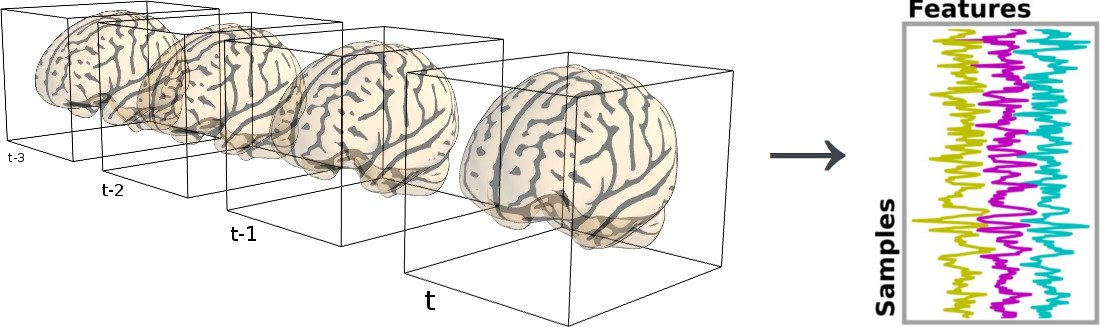
\includegraphics[width=.5\linewidth]{niimgs.jpg}
    \end{center}
    \caption{Conversion of brain scans into 2-dimensional data}
    \label{fig:niimg}
\end{figure}

Applying the mask is made easy by NumPy fancy indexing using boolean arrays.
Two-dimensional masked data will be referred to as \texttt{X} to follow
scikit-learn conventions:
\begin{lstlisting}
mask = nibabel.load('mask.nii').get_data()
func_data = nibabel.load('epi.nii').get_data()
# Ensure that the mask is boolean
mask = mask.astype(bool)
# Apply the mask, X = timeseries * voxels
X = func_data[mask].T

# Unmask data
unmasked_data = numpy.zeros(mask.shape, dtype=X.dtype)
unmasked_data[mask] = X
\end{lstlisting}

\subsection{Data visualisation}

Across all our examples, voxels of interest are represented on an axial slice of
the brain. Some transformations of the original matrix data are required to match
matplotlib data format. The following snippet of code shows how to load and
display an axial slice overlaid with an activation map. The background is an
anatomical scan and highest voxels of the background are taken as artificial
activation map.

\begin{lstlisting}
# Load image
bg_img = nibabel.load('bg.nii.gz')
bg = bg_img.get_data()
# Keep values over 6000 as artificial activation map
act = bg.copy()
act[act < 6000] = 0.

# Display the background
plt.imshow(bg[..., 10].T, origin='lower', interpolation='nearest', cmap='gray')
# Mask background values of activation map
masked_act = np.ma.masked_equal(act, 0.)
plt.imshow(masked_act[..., 10].T, origin='lower', interpolation='nearest', cmap='hot')
# Cosmetics: disable axis
plt.axis('off')
plt.show()
\end{lstlisting}

Note that a background is needed to display partial maps. Overlaying two images
can be done thanks to the \texttt{numpy.ma.masked\_array} data structure.
Several options exist to enhance the overall aspect of the plot.
Some of them can be found in the full scripts provided with this paper
\footnote{\url{http://www.github.com/AlexandreAbraham/frontiers2013}}. It generally
boils down to a good knowledge of Matplotlib. Note that the Nipy package provides a
\texttt{plot\_map} function that is tuned to display activation maps (a
background is even provided if needed).

% This part has been removed because automatic masking is overly complicated and
% does not brinautomatic masking is overly complicated and does not bring much
% to the paper.

% \subsubsection{Automatically computing a mask}

% The simplest strategy to compute a mask is a binarization by a selected threshold.
% Due to the nature of the neuroimaging data, there exists some strategy to choose
% this threshold in order to obtain a decent segmentation.

% \alex{There is a reference for the method used in Nisl. We should put it there
% and in the code. Add a figure with an histogram to illustrate.}

% Multi subject computation is simply done by intersecting subjects maps
% relatively to a chosen threshold.

%\subsubsection{Label shifting}
%
%Functional MRI acquisition is not immediate: BOLD response peak occurs between 3
%and 5 seconds after the stimulus. We take this time shift into account by
%shifting values of the label array by an offset of 2 time repetition (about 5
%seconds).

% Functional MRI measures brain activity by using the Blood-Oxygen-Level-Dependent
% contrast (BOLD). In fact, like muscles, brain regions consume more oxygen and
% nutriments when stimulated. So when a part of the brain starts working,
% physiological mechanisms induce an oxygen-rich blood flood toward this
% particular region: this is called haemodynamic response.

% However, this reaction takes time, usually around 3-4 seconds. This is the
% duration between the event and the reaction observed in the brain. To be able to
% match these two events, we will sometimes have to shift our data. The number of
% scans that must be shifted depends on the TR (repetition time) of the data.
% Usually, we remove the first two scans of the data and the two last values of the
% labels (to keep an homogeneous length).

%\begin{lstlisting}
%X = X[2:]
%y = y[:-2]
%\end{lstlisting}

\section{Decoding the mental representation of objects in the brain}

In the context of neuroimaging, \textit{decoding} refers to learning a model
that predicts behavioral or phenotypic variables from brain imaging data. 
The alternative that consists in predicting the imaging data given external
variables, such as stimuli descriptors, is 
called \textit{encoding}~\citep{naselaris2011}. It is further discussed in the next 
section.

First, we illustrate decoding with a simplified version of the experiment presented in
\cite{haxby2001}. In the original work, visual stimuli from 8 different categories
are presented to 6 subjects during 12 sessions. The goal is to 
predict the category of the stimulus presented to the subject given the
recorded fMRI volumes. This example has already been widely analyzed
(\cite{hanson2004combinatorial}; \cite{detre2006multi}; \cite{otoole2007};
\cite{hanson2008brain}; \cite{hanke2009pymvpa}) and has become a reference
example in matter of decoding. For the sake of simplicity, we restrict the example
to one subject and to two categories, faces and houses.

As there is a \emph{target} variable $y$ to predict, this is a supervised
learning problem. Here $y$ represents the two object categories, a.k.a.
\emph{classes} in machine-learning terms. In such settings, where $y$
takes discrete values the learning
problem is known as \emph{classification}, as opposed to
\emph{regression} when the variable $y$ can take continuous values,
such as age.

Many classification methods are available in scikit-learn. In this
example we chose to
combine the use of univariate feature selection and Support Vector
Machines (SVM). Such a classification strategy is simple,
yet quite efficient when used on neuroimaging data.

\subsection{Feature selection: ANOVA F-Test}

After applying a brain mask, the data consist of 40\,000 voxels, here
the features, for only 1\,400 volumes, here the samples.
Machine learning with many more features than samples
is challenging, due to the so-called \emph{curse of dimensionality}.
Several strategies exist to reduce the number of features.
A first one is based on prior neuroscientific
knowledge. Here one could restrict the mask to occipital areas, where the visual
cortex is located. A second approach is a data-driven. Features
are evaluated individually with a univariate statistical test. The variables
having the most discriminative power are kept.

Scikit-learn offers a panel of strategies to select features. In supervised
learning, the most popular feature selection method is the
ANalysis Of VAriance (ANOVA) F-Test. 
The null hypothesis of this test is that the feature takes the same value
independently of the value of $y$ to predict.

After ranking the features, \verb!sklearn.feature_selection! proposes a panel
of feature selection strategies. One can choose to take a percentile of the features
(\verb!SelectPercentile!), or a fixed number of features (\verb!SelectKBest!).
All these objects are implemented as transformers (see
 section~\ref{scikitlearn}).
In the code below, the \verb!f_classif! function (ANOVA F-Test) along with
the selection of a fixed number of features is used.

\subsection{Classification: SVM}

A linear SVM for classification, \verb!sklearn.svm.SVC!,
finds the hyperplane that maximally
separates the samples belonging to the different classes.
It is said to maximize the \emph{margin}. Classifying a new sample boils
down to determining on which side of the hyperplane it lies. When employing a
linear kernel, the separating hyperplane is defined in the input
data space and its coefficients can be related to the voxels.
Such coefficients can therefore be visualized as an image (after
unmasking step described in~\ref{sec:unmasking})
where voxels with high values have more influence on the prediction
than the others (see figure~\ref{fig:haxby}).

\begin{lstlisting}
feature_selection = SelectKBest(f_classif, k=500)
clf = SVC(kernel='linear')
X_reduced = feature_selection.fit_transform(X)
clf.fit(X_reduced, y)
### Look at the discriminating weights
coef = clf.coef_
### Reverse feature selection
coef = feature_selection.inverse_transform(coef)
\end{lstlisting}

\subsection{Searchlight}
\label{searchlight}

Searchlight \citep{kriegeskorte2006} is a popular algorithm in the
neuroimaging community. It runs a predictive model on a spatial
neighborhood of each voxel and tests the out-of-sample prediction
performance as proxy measure of the link between the local brain activity
and the target behavioral variable. In practice, it entails performing
cross-validation of the model, most often an SVM, on voxels contained in
balls centered on each voxel of interest. The procedure amounts to
solving a large number of SVMs and can be computationally expensive.
Detailing an efficient implementation of this algorithm is beyond the
scope of this paper. However, the code, along with this example,
are available in the github repository.

\subsection{Results}

\begin{figure}[hbtp]
  \begin{center}
  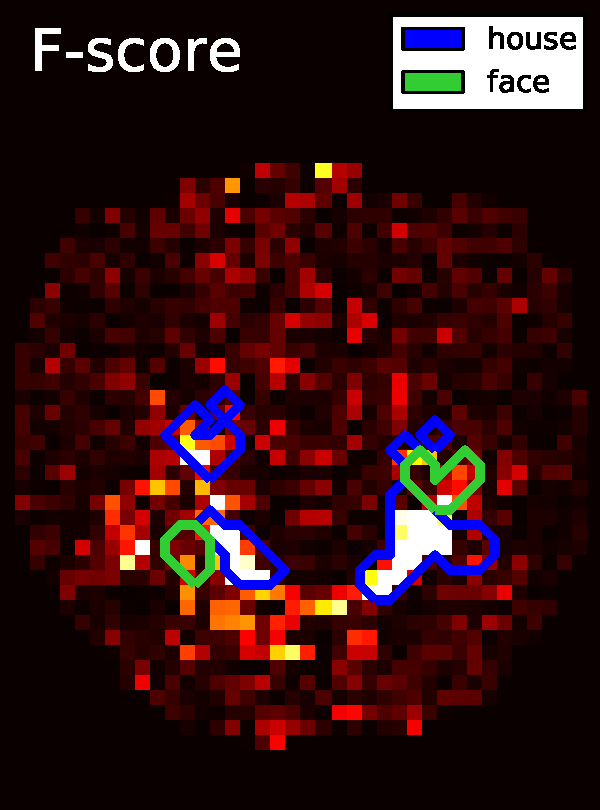
\includegraphics[width=.3\linewidth]{scripts/haxby/haxby_fscore}
  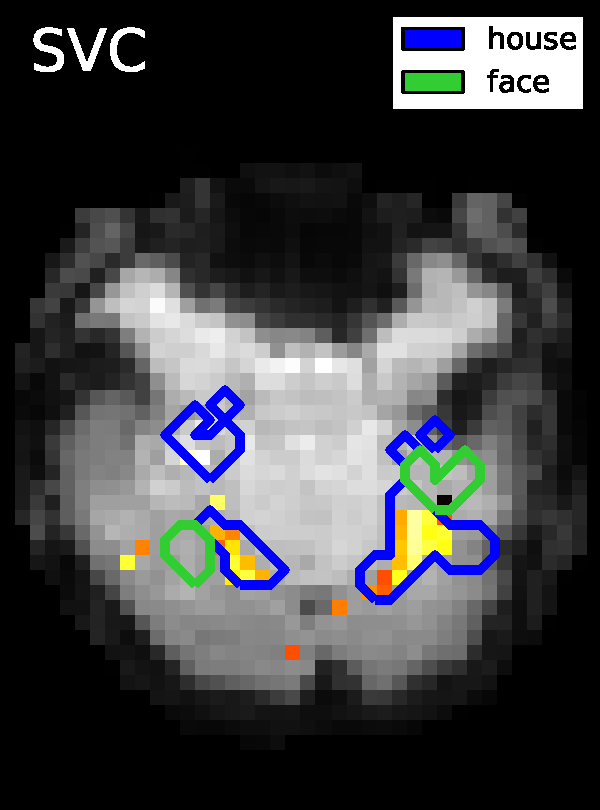
\includegraphics[width=.3\linewidth]{scripts/haxby/haxby_svm}
  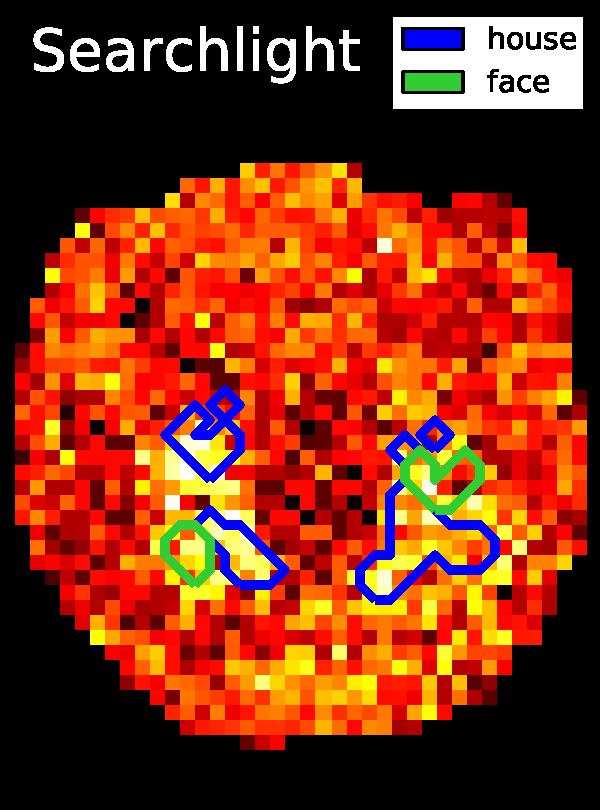
\includegraphics[width=.3\linewidth]{scripts/haxby/haxby_searchlight}
  \end{center}
\caption{Maps derived by different methods for face versus house
recognition in the Haxby experiment -- \emph{left}: standard analysis;
\emph{center}: SVM weights after screening voxels with an ANOVA; \emph{right}:
Searchlight map. The masks derived from standard analysis in the original
paper \citep{haxby2001} are displayed in blue and green.}
\label{fig:haxby}
\end{figure}

Results are shown in figure~\ref{fig:haxby}: first
F-score, that is standard analysis in brain mapping but also the
statistic used to select features; second the SVC weights after feature
selection and last the Searchlight map.
%
Note that the voxels with larger weights roughly match for all methods and
are located in the house-responsive areas as defined by the original paper.
%
The Searchlight is more expanded and blurry than the other methods
as it iterates over a ball around the voxels.

These results match neuroscientific knowledge as they highlight the
high level regions of the ventral visual cortex which is known to
contain category-specific visual areas. While Searchlight only gives a
score to each voxel, the SVC can be used afterward to classify unseen
brain scans.

Note that most of the example script \texttt{haxby\_decoding.py} is for data
loading and result visualization. Only 5 lines are needed to run a scikit-learn
classifier. Plus, thanks to the scikit-learn modularity, the SVC can be easily
replaced by any other classifier. The SearchLight estimator has been designed to
make use of any classifier and restrain the computation to an area of interest
for fast computation.


\section{Encoding brain activity and decoding images}
\label{kamitani}

In the previous experiment, the category of a visual stimulus was inferred from
brain activity measured in the visual cortex.
One can go further by inferring a direct link between the image
seen by the subject and the associated fMRI data.

In the experiment of \cite{miyawaki2008} several series of $10{\times}10$
binary images are presented to two subjects while activity on the visual cortex
is recorded.
In the original paper, the training set is composed of random images (where black and white pixels
are balanced) while the testing set is composed of structured images containing
geometric shapes (square, cross...) and letters. Here, for the sake of simplicity, we consider only the training set and use cross-validation to
obtain scores on unseen data.
%
In the following example, we study the relation between stimuli pixels and
brain voxels in both directions: the reconstruction of the visual stimuli
from fMRI, which is a decoding task, and the prediction of fMRI data
from descriptors of the visual stimuli, which is an encoding task.

\subsection{Decoding}

In this setting, we want to infer the binary visual stimulus presented to
the subject from the recorded fMRI data.
As the stimuli are binary, we will treat this problem as a classification
problem. Note that the method presented here cannot be extended as-is to
natural stimuli. 

In the original work, \cite{miyawaki2008} uses a Bayesian logistic regression
promoting sparsity along with a sophisticated multi-scale strategy.
As one can indeed expect the number of predictive voxels to be limited, we 
compare the $\ell_2$ SVM used above with
a Logistic Regression (LR) and a SVM
penalized with the $\ell_1$ norm
known to promote sparsity. The $\ell_1$ penalized SVM classifier compared here
uses a square-hinge loss while the LR uses a logit function.

% We ran a 5-fold cross validation to estimate the penalization parameter $C$
% (inverse of the amount of regularization); this yields the scores presented in
% figure~\ref{fig:miyawaki}.  % XXX : are you sure it's the figure you mean?

\begin{table}[htbp]
    \begin{center}
    \begin{tabular}{l|llllll}
        $C$ value           & 0.0005 & 0.001  & 0.005  & 0.01   & 0.05    & 0.1    \\
    \hline\\[-.9em]
    \hline\\[-.7em]
        $\ell_1$ Logistic Regression & 0.50 $\pm$ .02
                                     & 0.50 $\pm$ .02 
                                     & 0.57 $\pm$ .13
                                     & 0.63 $\pm$ .11
                                     & \textbf{0.70} $\pm$ .12
                                     & 0.70 $\pm$ .12 \\[.1em]
        $\ell_1$ SVC        & 0.50 $\pm$ .06
                            & 0.55 $\pm$ .12
                            & 0.69 $\pm$ .11
                            & \textbf{0.71} $\pm$ .12
                            & 0.69 $\pm$ .12
                            & 0.68 $\pm$ .12 \\[.1em]
        $\ell_2$ SVC        & 0.67 $\pm$ .12
                            & \textbf{0.67} $\pm$ .12
                            & 0.67 $\pm$ .12
                            & 0.66 $\pm$ .12
                            & 0.65 $\pm$ .12
                            & 0.65 $\pm$ .12
    \end{tabular}
    \end{center}
    \caption{5-fold cross validation accuracy scores obtained for different
    values of parameter $C$ ($\pm$ standard deviation).}
    \label{fig:miyawaki_cv}
\end{table}

Table~\ref{fig:miyawaki_cv} reports the performance of the different classifiers
for various values of C using a 5-fold cross-validation.
We first observe that setting the parameter $C$ is
crucial as performance drops for inappropriate values of C. It is particularly
true for $\ell_1$ regularized models. However,
in accordance with our prior knowledge, $\ell_1$
regularized models, when properly
parametrized, outperform an $\ell_2$ regularized estimator.
Both $\ell_1$ LR and SVM yield similar performances,
which is not surprising as they implement similar models.

\begin{lstlisting}
from sklearn.linear_model import LogisticRegression as LR
from sklearn.cross_validation import cross_val_score

pipeline_LR = Pipeline([('selection', SelectKBest(f_classif, 500)),
                        ('clf', LR(penalty='l1', C=0.05)])

scores_lr = []
# y_train = n_samples x n_voxels
# To iterate on voxels, we transpose it.
for pixel in y_train.T:
    score = cross_val_score(pipeline_LR, X_train, pixel, cv=5)
    scores_lr.append(score)
\end{lstlisting}




\subsection{Encoding}
Given an appropriate model of the stimulus, e.g. one which can provide an
approximately linear representation of BOLD activation, an encoding approach
allows one to quantify for each voxel to what extent its variability is captured
by the model. A popular evaluation method is the predictive \(r^2\) score, which
uses a prediction on left out data to quantify the decrease in residual norm 
brought about by fitting a regression function as opposed to fitting a constant. 
%We have \[r^2 = \frac{\|y_{\textrm{true}} - y_{\textrm{pred}}\|^2}{\|y_{\textrm{true}} - \bar y_{\textrm{true}}\|^2}\]
The remaining variance consists of potentially unmodelled, but reproducible signal
and spurious noise.

On the Miyawaki dataset, we can observe that mere black and white pixel values
can explain a large part of the BOLD variance in many visual voxels. Sticking
to the notation that \(X\) represesents BOLD signal and \(y\) the stimulus, we
can write an encoding model using the ridge regression estimator:

\begin{lstlisting}
from sklearn.linear_model import Ridge
from sklearn.cross_validation import KFold

cv = KFold(len(y_train), 10)
# Fit ridge model, calculate predictions on left out data
# and evaluate r^2 score for each voxel
scores = []
for train, test in cv:
    pred = (Ridge(alpha=100.).fit(y_train[train], X_train[train])
                             .predict(y_train[test]))
    X_true = X_train[test]
    scores.append(
        1. - ((X_true - pred) ** 2).sum(axis=0) /
        ((X_true - X_true.mean(axis=0)) ** 2).sum(axis=0))

mean_scores = np.mean(scores, axis=0)
\end{lstlisting}

\subsubsection{Receptive fields}
Given the retinotopic structure of early visual areas, it is expected
that the voxels well predicted by the presence of a black or white pixel
are strongly localized in so-called population
receptive fields (\textit{prf}). This suggests that only very few
stimulus pixels should suffice to explain the activity in each brain
voxel of the posterior visual cortex.
%
This information can be exploited by using a sparse linear
regression --the Lasso-- to find the receptive fields~\citep{tibshirani:96}.
Here we use the \emph{LassoLarsCV} estimator that relies on the LARS
algorithm~\citep{Efron04leastangle} and
cross-validation to set the Lasso parameter.

\begin{lstlisting}
from sklearn.linear_model import LassoLarsCV

# choose number of voxels to treat, set to None for all voxels
n_voxels = 50
# choose best voxels
indices = mean_scores.argsort()[::-1][:n_voxels]

lasso = LassoLarsCV(max_iter=10)

receptive_fields = [lasso.fit(y_train, X_train[:, index]
        ).coef_.reshape(10, 10)
        for index in indices]

\end{lstlisting}
%y_train_centered = (y_train - y_train.mean(axis=0)) / y_train.std(axis=0)

\subsection{Results}

\label{sec:miyawaki_results}
Results are presented in figure~\ref{fig:miyawaki}. They show the relation
between a specific image pixel and four voxels of interest in the brain.
In decoding settings, Figures \textit{a} and \textit{c} show the classifier's weights as brain
maps for both methods. They both give roughly the same results and we can
see that the weights are centered in the V1 and nearby retinotopic areas.
Figures \textit{b} and \textit{d} show reconstruction
accuracy score using LR and SVM
(variable \texttt{mean\_scores} in the code above).
Both methods give almost identical results. 
As in the original work \citep{miyawaki2008}, reconstruction is more
accurate in the fovea.
This is explained by the higher density of neurons dedicated to
foveal representation in the primary visual area.

In encoding settings, figure~\ref{fig:miyawaki}.e shows classifiers
weights for encoding, that we interpret as receptive fields. We can
see that receptive fields of neighboring voxels are neighboring
pixels, which is an expected result as we know that primary visual
cortex directly encodes the geometric structure and contrast of visual
stimuli.

Both encoding and decoding analysis show a link between the selected
pixel and brain voxels. In the absence of ground truth, seeing that
different methods come to the same conclusion comes as face validity.
% XXX face validity?
% XXX I was as puzzled as you are when I read it
% http://en.wikipedia.org/wiki/Face_validity


\begin{figure}[hbtp]
  \begin{center}
    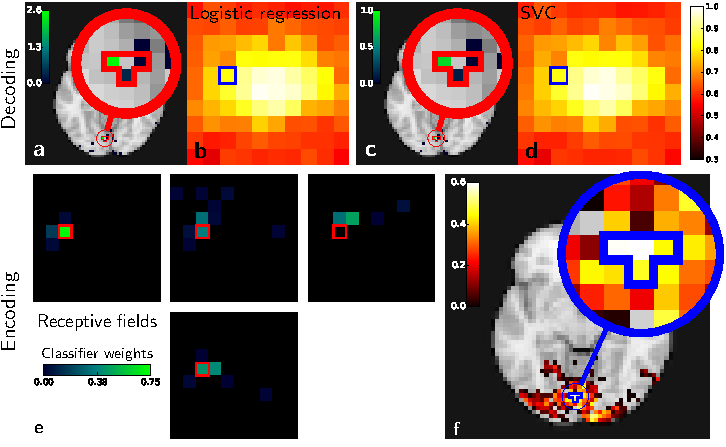
\includegraphics[width=\linewidth]{scripts/miyawaki/figure}
  \end{center}
  \caption{
      Miyawaki results in both decoding and encoding. Relations between one
      pixel and four brain voxels is highlighted for both methods.
      \textbf{Top: Decoding.} Classifier weights for the pixel
      highlighted (\textit{a.} Logistic regression, \textit{c.} SVM).
      Reconstruction accuracy per pixel
      (\textit{b.} Logistic
      regression, \textit{c.} SVM). 
      \textbf{Bottom: Encoding.} \textit{e}: receptive fields corresponding to
       voxels with highest scores and its neighbors.
       \textit{f}: reconstruction accuracy depending on 
	  pixel position in the stimulus. --- Note that the pixels and voxels highlighted are the same in 
      both decoding and encoding figures and that encoding and decoding
      roughly match as both approach highlight a relationship between the
      same pixel and voxels.
}
\label{fig:miyawaki}
\end{figure}


\section{Resting-state and functional Connectivity analysis}

Even in the absence of external behavioral or clinical variable, studying
the structure of brain signals can reveal interesting information.
Indeed, \cite{biswal1995} have shown that brain activation exhibits
coherent spatial patterns during rest. These correlated voxel activations
form functional networks that are consistent with known task-related networks.

Biomarkers found via predictive modeling on resting-state fMRI would be
particularly useful, as they could be applied to diminished subjects that
cannot execute a specific task. Here we use a dataset containing control
and ADHD (Attention Disorder Hyperactivity Disorder) patients resting
state data (subjects are scanned without giving them any specific task to
capture the cerebral background activity).

Resting state fMRI is unlabeled data in the sense that the brain activity
at a given instant in time cannot be related to an output variable.
In machine learning, this class of problems is known as unsupervised
learning. 
To extract functional networks or regions, we use methods that group together 
similar voxels by comparing their time
series. In neuroimaging, the most popular method is ICA and
is the subject of our first example. We will then show how to obtained 
functionally-homogeneous regions with
clustering methods.

\subsection{Independent Component Analysis (ICA) to extract networks}


ICA is a blind source separation method. Its principle is to separate a
multivariate signal into several components by maximizing their non-Gaussianity.
A typical example is the \emph{cocktail party problem} where ICA is able to separate
voices from several people using signal from microphones located across the room.

\subsubsection{ICA in neuroimaging}

ICA is the reference method to extract networks from resting state
fMRI \citep{kiviniemi2003}. Several strategies have been used to syndicate ICA
results across several subjects. \cite{calhoun2001a} propose a dimension
reduction (using PCA) followed by a concatenation of timeseries (used in this
example). \cite{varoquaux2010} use dimension reduction and canonical correlation analysis
to aggregate subject data. Melodic \citep{beckmann2004}, the ICA tool in
the FSL suite, uses a concatenation approach not detailed here.

\subsubsection{Application}

As data preparation steps, we not only center, but also detrend the time
series to avoid capturing linear trends with the ICA. Applying to the
resulting time series the FastICA algorithm~\citep{Hyvarinen:2000vk} with scikit-learn is
straightforward thanks to the transformer concept. The data matrix must
be transposed, as we are using \emph{spatial} ICA, in other words the
direction considered as random is that of the voxels and not the time
points. The maps obtained capture different components of the signal,
including noise components as well as resting-state functional networks.
To produce the figures, we extract only 10 components, as we are
interested here in exploring only the very large structures.

\begin{lstlisting}
# Here we start with Xs: a list of subject-level data matrices
# First we concatenate them in the time-direction, thus implementing
# a concat-ICA
X = np.vstack(Xs)
from sklearn.decomposition import FastICA
ica = FastICA(n_components=10)
components_masked = ica.fit_transform(data_masked.T).T
\end{lstlisting}

\subsubsection{Results}

On fig. \ref{fig:ica} we compare a simple concat ICA as implemented by
the code above to more sophisticated multi-subject methods, namely CanICA
and Melodic's concat ICA. We display here only the default mode network
as it is a well-known resting-state network. It is hard to draw conclusions from
a single map but, at first sight, it seems that both CanICA and Melodic
approaches are less subject to noise and give similar results.

\begin{figure}[hbtp]
  \centerline{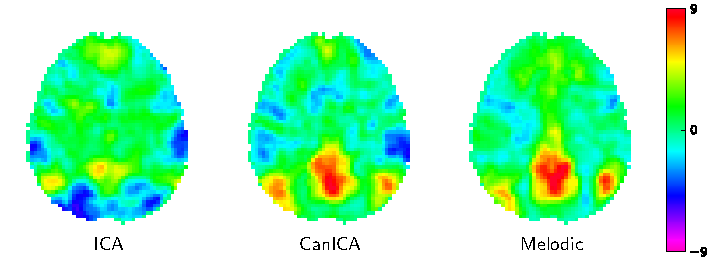
\includegraphics[width=.9\linewidth]{scripts/ica/figure}}
  \caption{Default mode network extracted using different approaches:
\emph{left}: the simple Concat-ICA approach detailed in this article;
\emph{middle}: CanICA, as implemented in nilearn; \emph{right}: Melodic's
concat-ICA.}
  \label{fig:ica}
\end{figure}

\subsection{Learning functionally homogeneous regions with clustering}
\label{clustering}

From a machine learning perspective, a clustering method aggregates 
samples into groups (called clusters) maximizing a measure of similarity
between samples within each cluster. If we consider voxels of a functional brain image
as samples, this 
measure can be based on functional similarity, leading to clusters of voxels
that form functionally homogeneous regions \citep{thirion2006}.

\subsubsection{Approaches}

Several clustering approaches exists, each one having its own pros and
cons. Most require setting the number of clusters extracted. This choice
depends on the application: a large number of cluster will give a more
fine-grained description of the data, with a higher fidelity to the
original signal, but also a higher model complexity. Some clustering
approaches can make use of spatial information and yield
spatially contiguous clusters, \emph{i.e.} parcels. Here we will describe
two clustering approaches that are simple and fast.

\paragraph{Ward clustering} uses a bottom-up hierarchical approach:
voxels are progressively agglomerated together into clusters. In
scikit-learn, structural information can be specified via a connectivity
graph given to the Ward clustering estimator. This graph is used to allow
only merges between neighboring voxels, thus readily producing contiguous
parcels. We will rely on the {\tt
sklearn.feature\_extraction.image.grid\_to\_graph} function to
construct such a graph using the neighbor structure of an image grid,
with optionally a brain mask.

\paragraph{K-means} is a more top-down approach, seeking cluster centers
to evenly explain the variance of the data. Each voxels are then assigned
to the nearest center, thus forming clusters. As imposing a spatial model
in K-means is not easy, it is often advisable to spatially smooth the
data.

To apply the clustering algorithms, we run the common data preparation
steps and produce a data matrix. As both Ward clustering and K-means rely
on second-order statistics, we can speed up the algorithms by reducing
the dimensionality while preserving these second-order statistics with a
PCA. Note that clustering algorithms group samples and that here we want
to group voxels. So if the data matrix is, as previously a (time points
$\times$ voxels) matrix, we need to transpose it before running the
scikit-learn clustering estimators. Scikit-learn provides a
\texttt{WardAgglomeration} object to do this \emph{feature agglomeration}
with Ward clustering \citep{michel2012supervisedclustering}, but this is
not the case when using K-Means.

\begin{lstlisting}
connectivity = grid_to_graph(n_x=mask.shape[0], n_y=mask.shape[1],
                             n_z=mask.shape[2], mask=mask)
ward = WardAgglomeration(n_clusters=1000, connectivity=connectivity)
ward.fit(X)
# The maps of cluster assignment can be retrieved and unmasked
cluster_labels = numpy.zeros(mask.shape, dtype=int)
cluster_labels[mask] = ward.labels_
\end{lstlisting}

\subsubsection{Results}

Clustering results are shown in figure~\ref{fig:clustering}. While
clustering extracts some known large scale structure, such as the
calcarine sulcus on fig~\ref{fig:clustering}.a, it is not guaranteed to
delineate functionally specific brain regions. Rather, it can be considered as a compression, that
is a useful method of summarizing information, as it groups together
similar voxels. Note that, as K-means does not extract spatially-contiguous
clusters, it gives a number of regions that can be much larger than the
number of clusters specified, although some of these regions can be very
small. On the opposite, Ward operates directly at the level of regions.
As it is a bottom-up process, it is often to be preferred when working
with a large number of clusters. There exist many more clustering
techniques expose in scikit-learn. Determining which is the best one to
process fMRI time-series requires defining more precisely the targeted
application.

\begin{figure}[hbtp]
  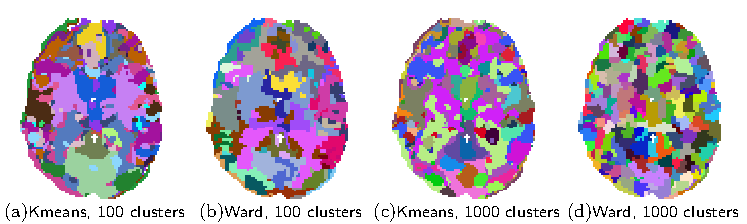
\includegraphics[width=\linewidth]{scripts/clustering/figure}
  \caption{Brain parcellations extracted by clustering. Colors are
random.}
  \label{fig:clustering}
\end{figure}

\section{Conclusion}

In this paper we have illustrated with simple examples how machine
learning techniques using the scikit-learn Python toolkit can be applied
to fMRI data in order to tackle
neuroscientific problems. Encoding and decoding can rely on supervised
learning to link brain images with stimuli. Unsupervised learning
can extract structure from resting-state data, functional networks or
brain regions. The accompanying Python code for the machine learning
tasks is very straightforward. Difficulties lie in applying proper 
preprocessing of the data, choosing the right model for the problem at
hand and interpreting these results. Tackling these difficulties while
providing the scientists with simple and readable code requires building
a domain-specific library, dedicated to applying scikit-learn to
neuroimaging data. This effort is underway in a nascent project, nilearn,
that aims to facilitate the use of scikit-learn on neuroimaging data.

Note that the examples described in this paper only scratch the
surface of the applications of statistical learning in neuroimaging. For
instance, sparse inverse covariance can extract the functional 
interaction structure from fMRI time-series \citep{varoquaux2013}, using
the graph-lasso estimator also available in scikit-learn.
Modern neuroimaging data processing entails fitting rich models on
limited data quantities. These are high-dimensional statistics problems
which call
for statistical-learning techniques. We hope that bridging a
general-purpose machine learning tool, scikit-learn, to domain-specific
data preparation code will open the door to new scientific advances.


\section*{Disclosure/Conflict-of-Interest Statement}
%All relationships financial, commercial or otherwise that might be perceived
%by the academic community as representing a potential conflict of interest
%must be described. If no such relationship exists, authors will be asked to
%declare that the research was conducted in the absence of any commercial or
%financial relationships that could be construed as a potential conflict of
%interest.
The authors declare that the research was conducted in the absence of any
commercial or financial relationships that could be construed as a potential
conflict of interest.

\paragraph{Funding\textcolon} We acknowledge funding from the NiConnect project.

\bibliographystyle{frontiersinSCNS} % for Science articles
\bibliography{biblio}

\end{document}
